% !TEX root = ../main.tex

\section{Bayesian Models as Program Code}
\label{sec:probprog:models}

In Section~\ref{sec:probprog:inv} we showed how one can think of PPS as inverting simulators, 
predicting internal variables given the outputs.  In this section we will take a 
different perspective and
show how we can translate Bayesian modeling into the framework of program code.   
In Chapter~\ref{chp:bayes} we showed how a Bayesian model is defined by a prior over
parameters and a likelihood function for those parameters given the data.  This viewpoint will
mostly translate into the probabilistic programming setting by equating between the prior
and sampling statements and between the likelihood and conditioning statements.  However,
in Section~\ref{sec:probprog:models:general} we will why explain why this is not always true
and suggest a formulation, distinct to that commonly used in the literature, for how the 
density implied by a query can be correctly represented.
%At the end
%of the section we will explain why this is actually a slight approximation (in short because we
%might condition on internally sampled variables) but for most purposes this viewpoint will suffice.
%We will keep things predominantly high-level for now, giving a more detailed look in
%Section~\ref{sec:probprog:anglican} by introducing a particular PPS, namely Anglican, in detail.

A key point to note throughout this section is that probabilistic programs define
models rather than procedures.  We refer to these models as \emph{queries}~\citep{goodman2008church} 
which are analogous to functions in a ordinary language.
In a standard programming language, functions take in inputs
and then run through a series of commands in order until termination is reached.\footnote{In functional
	programming languages operations are not necessary carried out in the order they are defined,
	but it still holds that the function takes inputs carries out a series of actions until the desired output
	is (perhaps lazily) calculated.}  Likewise, random sampling statements like {\small \texttt{rand}, \texttt{randn}}
etc, make a single independent draw from the same distribution each time they appear in the execution trace.
Neither is the case for a probabilistic program query.  Instead a  query defines a model
which is compiled to a form that can be interpreted by an inference engine which then
outputs some characterization of the posterior such as a series of samples.  Perhaps the easiest way to think
about how a probabilistic program language works (though not necessarily what happens for all systems) is that
the query is, or sometimes parts of the query are, run many times and the exact behavior
of this running is control by the inference engine.  For example, the inference engine 
might sample from a different distribution then specified by the original sampling statement or it
might run lots of instances of the query in parallel and then terminate some of the instances
performing poorly, while duplicating instances doing well.

\subsection{A Simplified Probabilistic Programming Setup}
\label{sec:probprog:models:first}

We first consider the case of constructing a restricted example PPL.  We emphasize that
this is by no means the only setup one can use, with design choices made in the interest of exposition.
We will presume that our PPL
has no branching (i.e. there are no \texttt{if} statements or equivalent), recursion, or memoization
(i.e. functions are always re-evaluated from scratch when called); is first order
(i.e. variables cannot be functions); and that it does not allow 
any conditioning on internally sampled variables.  
We will give our language
two special constructs, \sample and \observe, between which the distribution of the
query is defined. 
Informally, \sample will be used to specify terms in the prior and \observe terms in the
likelihood.  More precisely, \sample will be used to make random draws $x_t \sim f_t(x_t | \Xi_t)$,
where $\Xi_t$ is a subset of the variables in scope at the point of sampling, and \observe will use to condition on
data $g_s(y_s|\Lambda_s)$ with $\Lambda_s$ defined in the same way as $\Xi_t$.  
For our inference, it will be necessary to control the sampling and so we define
the syntax of \sample to take a \emph{distribution object} as its only input and for \observe
to take a distribution object and an observation as input.  We further define each distribution
object as containing a sampling procedure and a density function that can be evaluated
exactly.\footnote{It will actually often be possible to use incomplete distribution objects for
	both \sample and \observe that only contain the sampler and the density function respectively.
	This former can be permitted by using inference algorithms that use the prior as the proposal, such
	that only the sampler will be required.  The latter is sufficient in the vast majority of scenarios as, unless
	one is carrying out amortization~\citep{paige2016inference,le2017inference}, the data is fixed and does
	not need to be sampled.}  Our language will be provided with a number of \emph{elementary random
	procedures} in
the form of distribution classes for common sampling distributions such as the normal and Poisson
distributions, but will also provide the ability for users to define their own distribution classes.   These
classes allow a distribution object to be constructed when provided with the required parameters, such that
the distribution is fully defined before being passed to a \sample or \observe.
We complete our syntactic definition of \sample and \observe by defining them to return a sample and \texttt{nil}
respectively.
 We will presume here and throughout that, other than the effects of \sample and \observe,
 functions in our PPL are \emph{pure} such that they always provide the same outputs when
 called with the same inputs.  This restriction naturally means that queries should not have
 any random components other than dictated by \sample and \observe, but also suggests that
 they should be free from side effects such as modifications of global variables.

\begin{figure}[p]
	\centering
	\begin{subfigure}[t]{\textwidth}
		\centering	
		\begin{minipage}[t]{0.48\textwidth}
		\begin{algorithmic}[1]
			\renewcommand{\algorithmicrequire}{\textbf{Inputs:}}
			\renewcommand{\algorithmicensure}{\textbf{Outputs:}}			 
			\Require Student-t degrees of freedom $\nu$, error
			scale $\sigma$, data $y_{1:S} = \{u_s,v_s\}_{s=1}^S$
			%\Ensure weighted samples $\left\{x_{1:T}^i,w_T^i\right\}_{i=1}^N$
%			\State \texttt{m\_dist} $\leftarrow$ 
%			\State \texttt{c\_dist} $\leftarrow$ \normal(0,1)
			\State $m\leftarrow$\sample(\normal(0,1))
			\State $c\leftarrow$\sample(\normal(0,1))
			\State \lstinline$obs-dist$\xspace $\leftarrow$ \studentt $(\nu)$
			\For{$s=1,\dots,S$}	
			\State $d \leftarrow (v_s-m u_s - c)/\sigma$
			\State \observe(\lstinline$obs-dist$\xspace,~$d$)
			\EndFor
			\State \Return $m, \; c$
		\end{algorithmic}
		\end{minipage}
		~~
		\begin{minipage}[t]{0.48\textwidth}
			\vfill
			\resizebox{\textwidth}{!}{
				% !TEX root = ../../main.tex

\begin{tikzpicture}

\node[latent, minimum size=27pt] (m) {$m$};
\node[latent, right=1.4cm of x1, minimum size=27pt] (c) {$c$};

\node[obs, below=of m, minimum size=27pt, xshift=-2.7cm] (y1) {$y_1$};
\node[obs, right=1cm of y1, minimum size=27pt] (y2) {$y_2$};
\node[right=1cm of y2, minimum size=27pt] (y3) {{\tiny $\bullet \; \bullet \; \bullet$}};
\node[obs, right=1cm of y3, minimum size=27pt] (y4) {$y_{S\text{-}1}$};
\node[obs, right=1cm of y4, minimum size=27pt] (y5) {$y_S$};

\edge {m,c} {y1,y2,y4,y5};

\end{tikzpicture}}
			{\small
			\begin{align*}
			p(m,c&, y_{1:S} | \nu, \sigma)= \mathcal{N}(m;0,1) \; \mathcal{N}(c;0,1) \\
										&\prod_{s=1}^{S} \textsc{Student-T} \left(\frac{v_s-mu_s-c}{\sigma} ; \nu \right)
			\end{align*}}
		\end{minipage}
		\caption{Bayesian linear regression model with student-t likelihood, namely
			$v_s = m u_s + c + \sigma \epsilon_s$ where $\epsilon_t \sim \textsc{Student-T}(\nu)$.
			We presume that the scaling of the error $\sigma$ and the number of degrees of freedom $\nu$
			are fixed input parameters (i.e. $\phi=\{\nu,\sigma\}$), that our fixed data is $y_{1:S} = \{u_s,v_s\}_{t=1}^S$,
		 and that we are trying to infer the slope $m$ and intercept $c$ (we thus have $x_1=m$, $x_2=c$ in our
		 general notation), both of which are assigned a unit Gaussian as a prior.  Our query
			first samples $m$ and $c$ (note that \normal(0,1) generates a unit Gaussian distribution object)
			and constructs a student-t distribution object \lstinline$obs-dist$.  It then cycles
		  over each datapoint and observes $(v_t-m u_t -c)/\sigma$ using \lstinline$obs-dist$,
		  before finally returning $m$ and $c$ as outputs.  
%		  The query corresponds to the graphical model
%		  shown in the top right and induces the joint distribution shown bottom right.  
		  Note that if we instead
		  wished to directly predict the outputs at some untested inputs points $u_{S+1:S+n}$ then we could
		  predict these anywhere in the query (after $m$ and $c$ have been defined) and return these
		  as outputs along with, or instead of, $m$ and $c$.
		  \label{fig:probprog:linear-reg}
		  }
	\end{subfigure}
		\begin{subfigure}[t]{\textwidth}
			\vspace{10pt}
\centering	
\begin{minipage}[t]{0.45\textwidth}
	\begin{algorithmic}[1]
		\renewcommand{\algorithmicrequire}{\textbf{Inputs:}}
		\renewcommand{\algorithmicensure}{\textbf{Outputs:}}			 
		\Require Transition std-dev $\sigma$, output shape $\alpha$,
		output rate $\beta$, data $y_{1:T}$
		%\Ensure weighted samples $\left\{x_{1:T}^i,w_T^i\right\}_{i=1}^N$
		%			\State \texttt{m\_dist} $\leftarrow$ 
		%			\State \texttt{c\_dist} $\leftarrow$ \normal(0,1)
		\State $x_0\leftarrow0$
		\State \lstinline$tr-dist$\xspace $\leftarrow$ \normal $(0,\sigma)$
		\State \lstinline$obs-dist$\xspace $\leftarrow$ \lstinline$gamma$\xspace $(\alpha,\beta)$
		\For{$t=1,\dots,T$}	
		\State $x_t \leftarrow x_{t\text{-}1}+$\sample(\lstinline$tr-dist$\xspace)
		\State \observe(\lstinline$obs-dist$\xspace,~$y_t-x_t$)
		\State $z_t \leftarrow \mathbb{I}(x_t>4)$
		\EndFor
		\State \Return $z_{1:T}$
	\end{algorithmic}
\end{minipage}
~~
\begin{minipage}[t]{0.52\textwidth}
	\vspace{-6pt}
	~~~\resizebox{0.96\textwidth}{!}{
		% !TEX root = ../../main.tex

\begin{tikzpicture}

\node[latent, minimum size=27pt] (x1) {$x_1$};
\node[latent, right=1cm of x1, minimum size=27pt] (x2) {$x_2$};
\node[right=1cm of x2] (x3) {{\tiny $\bullet \; \bullet \; \bullet$}};
\node[latent, right=1cm of x3, minimum size=27pt] (x4) {$x_{T\text{-}1}$};
\node[latent, right=1cm of x4, minimum size=27pt] (xT) {$x_T$};

\node[obs, below=1cm of x1, minimum size=27pt] (y1) {$y_1$};
\node[obs, below=1cm of x2, minimum size=27pt] (y2) {$y_2$};
%\node[obs, below=of x3] (y3) {$y_3$};
\node[obs, below=1cm of x4, minimum size=27pt] (y4) {$y_{T\text{-}1}$};
\node[obs, below=1cm of xT, minimum size=27pt] (yT) {$y_T$};

%\node[latent, above=of x1, xshift=-1.2cm, minimum size=27pt] (t) {$\theta$};

\edge {x1} {x2,y1} ; %
\edge {x2} {x3,y2} ; %
\edge {x3} {x4} ; %
\edge {x4} {xT,y4} ; %
\edge {xT} {yT} ; %

%\edge {t} {x1,x2};
%\edge[bend left=0] {t} {x4};
%\edge[bend left=10] {t} {xT};

\end{tikzpicture}}
	{\small
	\begin{align*}
	p&(x_{1:T}, y_{1:T} | \sigma,\alpha,\beta)= \\
	&\mathcal{N}(x_1;0,\sigma^2) \; \textsc{Gamma}(y_1-x_1;\alpha,\beta)\\
	&\prod_{t=2}^{T} \mathcal{N}(x_t-x_{t-1};0,\sigma^2) \; \textsc{Gamma} (y_t-x_t;\alpha,\beta)
	\end{align*}}
\end{minipage}
			\caption{State-space model with Gaussian transition and Gamma emission distributions.
				It is a form of the HMM model given in~\eqref{eq:bayes:hmm} with
				$p(x_1)=\mathcal{N}(x_1;0,\sigma^2)$, $p(x_t | x_{t-1}) = \mathcal{N}(x_t-x_{t-1}; 0,\sigma^2)$,
				and Gamma likelihood model $p(y_t | x_t) = \textsc{Gamma}(y_t-x_t ; \alpha, \beta)$ with
				shape parameter $\alpha$ and scale parameter $\beta$.  We assume that the input
				parameters $\phi = \{\sigma,\alpha,\beta\}$ are fixed and we want
				to sample from $p(z_{1:T} | y_{1:T}, \phi)$ given data $y_{1:T}$, where each 
				$z_t$ is an indicator for if $x_{t}$ exceeds a threshold of $4$. Our query, exploiting the
				equivalence between $p(x_1)$ and $p(x_t|x_{t-1}=0)$, first initializes $x_0=0$ and creates
				distribution objects for the transitions \lstinline$tr-dist$\xspace and emissions
				\lstinline$obs-dist$\xspace.  It then loops over time steps, sampling each $x_t$ given
				$x_{t-1}$, observing $y_t$ given $x_t$, and deterministically calculating $z_t$.  Finally
				the $z_{1:T}$ are returned as the desired output.
				\label{fig:probprog:LGSSM}
				}
		\end{subfigure}
\caption{Example pseudo-queries for our simplified probabilistic programming setup with
	corresponding graphical models and joint distributions.\label{fig:probprog:example-progs}}
\end{figure}

For our simplified setup, we distinguish between two types of inputs to our queries: external 
parameters $\phi$ and data $y_{1:S}$.
The external parameters are defined as the inputs that are 
not ``observed'' at any point but can effect the conditioning through $\Xi_t$ and $\Lambda_s$.
We presume that the data terms, defined as the inputs we are observed, 
appear in neither $\Xi_t$ or $\Lambda_s$.
We now define both \sample and \observe from the probability model perspective
as adding a factor to the joint distribution which is therefore given by
\begin{align}
\label{eq:probprog:simple-joint}
p(x_{1:T},y_{1:S} | \phi) = \prod_{t=1}^{T} f_t(x_t | \Xi_t) \prod_{s=1}^{S} g_s(y_s|\Lambda_s).
\end{align}
The two vary in whether they define a new random variable (\sample) or effect the probability of the
query given particular instances of the other random variables (\observe).
Our presumptions for this simplified setup that no $y_{s}$ terms are present in the $\Xi_t$ or $\Lambda_s$
and that we do not condition on internally sampled variables, means that the product of the \sample terms
correspond exactly to our prior $\prod_{t=1}^{T} g_t(x_t | \Xi_t) =: p(x_{1:T} | \phi)$ and that the
product of the \observe terms corresponds exactly to our likelihood
$\prod_{s=1}^{S} g_s(y_s|\Lambda_s) =: p(y_{1:S} | x_{1:T}, \phi)$.  Consequently, for our simplified setup,
each query defines a finite directed acyclic graphical model (see Section~\ref{sec:bayes:paradigm:graph})
where the conditional relationships are defined through the definitions of $f_t$ and $g_s$.
This breakdown into a prior and likelihood and the equivalence to graphical models
will not hold in the more general cases we consider later.  Our aim will be to perform inference
to provide a characterization of $p(x_{1:T} | y_{1:S}, \phi)$ (or the posterior for some deterministic
mapping of $x_{1:T}$), typically in the form of (approximate)
samples.  Figure~\ref{fig:probprog:example-progs} shows two example queries
along with the corresponding graphical models and joint distributions they define.

Other than \sample and \observe statements, the rest of our query is by construction totally deterministic.  Therefore,
though it may contain random variables other than $x_{1:T}$, these random variables are deterministic
functions of the ``raw'' random draws $x_{1:T}$ and inputs $\phi$ and $y_{1:S}$.  We can therefore 
define the outputs of our query as $\Omega := h(x_{1:T},y_{1:S},\phi)$ for some deterministic function $h$.
As we explained in Section~\ref{sec:prob:measure}, the change of variables means that the density function on $\Omega$,
$p(\Omega | y_{1:S}, \phi) $
can have a different form to the posterior implied by our query, namely $p(x_{1:T} | y_{1:S}, \phi)$.
  Though this is a serious complication in the
context of optimization (we may not in general be able to find $\argmax_{\Omega} p(\Omega|y_{1:S},\phi)$
or even evaluate $p(\Omega | y_{1:S}, \phi)$ exactly), it
is perfectly acceptable in the context of calculating expectations as
\begin{align}
\int f(\Omega) p(\Omega | y_{1:S}, \phi) d\Omega = \int f(h(x_{1:T}, y_{1:S}, \phi)) p(x_{1:T} | y_{1:S}, \phi) dx_{1:T}
\end{align}
for implicitly defined measures $d\Omega$ and $dx_{1:T}$.  One consequence of this is that
we can express any expectations calculated by our query as expectations over $p(x_{1:T} | y_{1:S}, \phi)$
which was fully defined by the joint~\eqref{eq:probprog:simple-joint}.  Another is that, provided we are not worried
about carrying out optimizations, we do not need to explicitly worry about the implicit measures defined
by the definition of our query, other than any potential effects on the inference scheme.  In particular,
if our aim is to generate samples from $p(\Omega | y_{1:S}, \phi)$ then
we can simply generate samples from $p(x_{1:T} | y_{1:S}, \phi)$ and deterministically convert each
sample to the space of $\Omega$.  In other words, our inference engine does not need to worry about
the consequences of changes of variables if our intended output is just a sequence of samples.

An important point to note is that~\eqref{eq:probprog:simple-joint} shows that all of our \sample
and \observe statements are exchangeable, in the sense that their order can be moved around and
still define the same joint distribution, up to restrictions about all the required variables (namely the
distribution object and, if required, observation in our current setup) existing and being in scope.  
For example, if all variables remain in scope
and are not redefined, we can generally move all our \observe statements to the end of the query
without changing the joint distribution.  Therefore the query given in Figure~\ref{fig:probprog:LGSSM}
would define the same model if all the $x_t$ were sampled upfront before making any observations.
Nonetheless, the position of the \observe statements
can often be important from the perspective of the performance of the inference engine.  This exchangeability
result will carry over to the non-simplified case.

%
%Because of the assumptions we have made for our language, the latent
%variables we wish to do inference for are statically determined as $x_{1:T} = x_1,\dots,x_T$ 
%such that the posterior of interest is $p_{\phi} (x_{1:T} | y_{1:S})$ (or some marginal of this for
%which we can still using Monte Carlo inference on the joint).
%
%Our implied target posterior
%is proportional to this joint in the standard way $p_{\phi}(x_{1:T}|y_{1:S}) \propto p_{\phi}(x_{1:T},y_{1:S})$.

\subsection{A General Probabilistic Programming Setup}
\label{sec:probprog:models:general}

Perhaps surprisingly, we do not need to do anything to our language to extend it to a universal
PPL other than to relax a number of the restrictions made for our simplified case.  Namely,
we will allow branching, higher order functions, (potentially infinite) recursion, stochastic memoization~\citep{goodman2008church},
conditioning on internally sampled
variables, and the use of the ``data'' inputs $y_{1:T}$ in the definition of our generate model (instead of
just allowing them to be observed).  We will maintain the syntax of our simplified
setup, along with the assumption that functions are pure other than the effect of \sample and \observe.
An important point to note though for why such a language is universal, is that arbitrary distributions
with countable parameters can be defined through a series of uniform $[0,1]$ draws followed
by an arbitrary deterministic mapping -- after all, this is effectively how all probability distributions are
defined from a measure theoretic point of view.\footnote{Interesting, this viewpoint breaks down for
	distributions over functions for which measure theory itself somewhat breaks down~\cite{heunen2017convenient}.
	As such, universal PPSs actually go beyond the standard measure-theoretic view of probability.}

Despite their ostensibly modest nature,
these generalization will have a substantial effect on the intuitions relating our universal
PPL to the Bayesian framework, the range of models we can define, and the difficulty of performing
general purpose inference.  For example, as $y_s$ terms can appear in the $\Xi_t$ terms,
it can be the case that $p(x_{1:T} | \phi) \neq \prod_{t=1}^{T} p(x_t | \Xi_t)$, such that the latter no
longer explicitly corresponds to a conventional definition of a prior.  Some variables may change type (e.g.
between continuous and discrete) or even not exist depending on the value of other variables.  The number
of variables may change from one execution to the next and it could even be the case that the number
of latent variables is unbounded provided that any possible execution has a 
finite number of variables is with probability $1$, such
as is the case for certain Bayesian non-parametric models such as the Dirichlet process~\citep{ferguson1973bayesian,teh2011dirichlet}.
Note that the number \sample and \observe statements lexically defined within our query must,
for obvious reasons, be finite, but recursion or looping may mean that they are evaluated an uncountable
number of times.  It is also possible for a variable within a query to itself encode an
infinite number of parameters, for example, one might include a Gaussian process within the query (see Section~\ref{sec:opt:GPs}).
These complications make it difficult to mathematically reason about the joint distribution defined by a query in a
universal PPS, let alone reason about its breakdown into a prior and a likelihood or represent the query
using a graphical model (which might actually not even be possible).

One way to conceptually overcome these difficulties is to reason in terms of \emph{execution paths}.
Even though we might not know upfront which \sample and \observe statements are invoked by
a particular query output, if we execute the query in order, the draws of the \sample statements made
thus far in an \emph{execution trace} uniquely identify which \sample statement will be invoked next and
the value of all the variables up
to that \sample statement.
In other words, given the outcome of $t$ evaluated \sample statements, which \sample statement corresponds
to the $(t+1)$-th to be evaluated is uniquely defined and the query up to that \sample statement is
completely deterministic, including which path to take at each \texttt{if} statement, which variables are defined
and their values, and the probability arising from the \observe conditioning statements.\footnote{Note that our
	inference algorithm might induce probabilistic behavior at \observe statements, but we can ignore this
	is terms of defining the distribution defined by the query.}
Thus although the distribution of the query is not necessarily statically
determinable, it can still be \emph{evaluated through execution} as each \sample statement provides
the information we require, in addition to the information from the previous \sample statements, to deterministically evaluate
up to the next \sample statement.
Consequently, we can evaluate the probability of any particular trace as we run it, even though it might
be challenging to evaluate the probability of a predefined configuration of the variables.

Using this idea of execution paths, we can define an expression for the conditional probability a query defines,
albeit in a complex and somewhat abstract manner that only really retains meaning in our probability calculation through
evaluation mindset, by defining the probability of a particular trace.  First let $\lambda$ denote all the 
inputs to the query (including both parameters and
data as we will now have no explicit distinction between the two).  Further let
$n_x$ and $n_y$ be the number of \sample and \observe statements
respectively invoked by the trace, noting that $n_x$ and $n_y$ may themselves be random variables and could
potentially be unbounded (e.g. $n_x$ could follow a Poisson distribution).
We can now define, for any given execution, $x_{1:n_x} = x_1,\dots,x_{n_x}$ and $y_{1:n_y} = y_1,\dots,y_{n_y}$ respectively as the
outputs of our $n_x$ \sample statements and observation inputs for our $n_y$ \observe statements.
To avoid complications regarding variable reassignment, we will not consider the $x_j$ as being variables
in our program, such that calling $a \leftarrow$\clj{sample(dist)} effectively creates an internal protected variable $x_j$
(whose value can never be reassigned) and then immediately assigns the value of $x_j$ to $a$.
All variables generated before $x_{j}$ are a deterministic function of $x_{1:j-1}$ and $\lambda$.  Therefore, 
even though all variables in our program might be random, including the observations $y_k$, all
are deterministically calculable given $x_{1:n_{x}}$ and $\lambda$.  Even $n_x$ itself is a deterministic function
of the output of the \sample statements, as $\{x_{1:j},\lambda\}$ deterministically dictates whether there will be any
further \sample statements encountered.  Consequently, in the same way
we only needed to worry about $x_{1:n_x}$ to reason about the distribution over the program outputs for
our simplified case, we can reason about the distribution on all variables in program through $x_{1:n_x}$ in our
general case for a given $\lambda$.  We can thus think of our trace as being defined by $\xnx$.

We continue by defining $f_{1},\dots,f_{n_s}$ and $g_{1},\dots,g_{n_o}$ respectively as the densities (with respect to
an implicitly defined measure) associated with the $n_s$ \sample 
and $n_o$ \observe statements defined lexically within a raw program code (i.e. the distinct \sample and \observe
statements appearing anywhere in the raw program code), noting that $n_s$ and $n_o$ are \emph{not} random variables.
To express these densities, we use the notation $f_i(x_j|\eta_j)$ 
to indicate the density of lexical \sample statement $i$ returning outputs $x_j$ when provided
with distribution object $\eta_j$, which will typically be a random variable itself.  Note here that parameters
of the density are encoded through the distribution object, so for example we can think of
\sample(\normal($\mu,1$)) for a random variable $\mu$ as first creating the random distribution object
$\eta_j=$\normal($\mu,1$) before passing this to the \sample call.
We similarly use the notation $g_i(y_k|\psi_k)$ to express the density of
using lexical \observe $g_i$ to observe output $y_k$ with the (random) distribution object $\psi_k$.
We define $a_j \in \{1,\dots,n_s\}, \; 
\forall j\in\{1,\dots,n_x\}$ and $b_k \in \{1,\dots,n_o\}, \; \forall k\in\{1,\dots,n_y\}$ as the
random variables respectively used to index which of the lexical \sample and \observe statements
correspond to the $j^{\text{th}}$ and $k^{\text{th}}$ execution trace \sample and \observe statements.

To encapsulates the notion of a valid trace, we define the deterministic boolean function $\mathcal{B}(x_{1:n_x},\lambda)$
which returns $1$ if the trace is valid and $0$ otherwise.   This is something we do not need
to worry about if we take an evaluation based inference approach, whereby
we rely on methods that only simulate from the generative model, but it is necessary to ensure that the density
is well defined if we try to evaluate it at a predetermined point, chosen externally to the program.
For example, $\mathcal{B}(x_{1:n_x},\lambda)$ is necessary to
ensure that $x_{1:n_x}$ is a ``complete'' trace: it may be that a certain $x_{1:n_x}$
implies that further \sample statements are still to be invoked after the $n_x^{\text{th}}$ in which case the
trace is not valid as these additional outputs are undefined.  For example, if the program defines the distribution
$\mathcal{N}(x_1;0,1)\mathcal{N}(x_2;0,1)\mathcal{N}(4;x_2,x_1)$, then the trace $x_1=3.2$ is incomplete
and although there is well defined marginal on $x_1$, its density in general not equal to that implied by
partial evaluation of the trace.  
Similarly, we can use  $\mathcal{B}(x_{1:n_x},\lambda)$ to encode that in our example $P(n_x>2)=0$.  Meanwhile,
$\mathcal{B}(x_{1:n_x},\lambda)$ also ensures that  all terms within the
trace probability are well defined.  For example, an invalid trace might provide parameters of the wrong type
to one of the distribution objects, meaning that density of that distribution object is undefined.

We now finally define the conditional distribution on the trace $\mT$
implied by our query as $p(\mT = x_{1:n_x} | \lambda)
\propto \gamma(x_{1:n_x}, \lambda)$ where
\begin{align}
\label{eq:probprog:universal-cond}
\gamma(x_{1:n_x}, \lambda) = \begin{cases}
\prod_{j=1}^{n_x} 
f_{a_j}(x_j | \eta_j)
\prod_{k=1}^{n_y}
g_{b_k}(y_k | \psi_k) \quad \text{if} \quad \mathcal{B}(x_{1:n_x},\lambda)=1 \\
0 \quad \text{otherwise}
\end{cases},
\end{align}
remembering that although the $a_j$, $\eta_j$, etc are random variables, they are all deterministically
calculable from $x_{1:n_x}$ for a given query and $\lambda$.  
%Similarly $\mathcal{B}(x_{1:n_x},\lambda)$
%is a deterministic function implied by the program.
 As a consequence, our program implies a well
defined, normalized, conditional distribution, or ``posterior, on the produced traces
(presuming the normalization constant is finite and non-zero). 
Note that this definition is
explicitly on outcomes of the trace and so, in general, $p(\mT = x_{1:j} | \lambda) \neq
\int p(\mT = x_{1:n_x} | \lambda) dx_{j+1:n_x}$.  In fact, it is always necessary that at least one of
$p(\mT = x_{1:j} | \lambda)$ and $p(\mT = x_{1:n_x} | \lambda)$ are equal to zero if they share the
same $x_{1:j}$, as it is not possible to have $\mathcal{B}(x_{1:n_x},\lambda)=\mathcal{B}(x_{1:j},\lambda)=1$.

An illustrative example for calculating the probability of a program through execution traces
for a problem that cannot not be expressed using our simplified PPL or a graphical model, but
which is simple to write in our universal framework, is shown in Figure~\ref{fig:probprog:poisson}.
Imagine we want to calculate the unnormalized trace probability
$\gamma(x_{1:n_x}=[0.2,0.07],\lambda=4)$ which we can do by stepping through the program and accumulating
terms (for reference we will be following the cyan path
in Figure~\ref{fig:probprog:poi-traces}).  
On our path we first hit $f_1(x_1 | \eta_1) = \textsc{Uniform}(0.2;0,1) = 1$, we fix $u\leftarrow x_1$
and $p\leftarrow 1\cdot u$, and test if $p=0.2\le \exp(-4) \approx 0.0183$.  This gives false
and so we do not break the while loop, instead encountering
$g_2(y_1 | \psi_1) = \textsc{Bernoulli}(1;0.2) = 0.2$ and so our running value for
$\gamma(x_{1:n_x}=[0.2,0.07],\lambda=4)$ is $1\times0.2 = 0.2$.  Updating $k\leftarrow1$ and
going back to the
start of the while loop we encounter $f_1(x_2 | \eta_2) = \textsc{Uniform}(0.07;0,1) = 1$,
so our running score is $1\times0.2\times1=0.2$.
Reassigning $u$ and $p$ we see that  $p=0.014\le \exp(-4)$ is now true and so we take
the opposite branch to before with our if statement, thus breaking the while loop.  To
finish the program we pass through $g_1(y_2 | \psi_2) = \textsc{Bernoulli}(k>3;0.99) = 0.01$
giving the final unnormalized density of $\gamma(x_{1:n_x}=[0.2,0.07],\lambda=4)=0.002$ and an output of $k=1$.
We finish by checking that our trace was valid, which we can easily see is the case because
no terms were undefined and we generated the correct number of sample outputs (i.e. $n_x=2$ as
required).

\begin{figure}[p]
	\centering
	\vspace{-10pt}
	\begin{minipage}[t]{\textwidth}
		\centering
		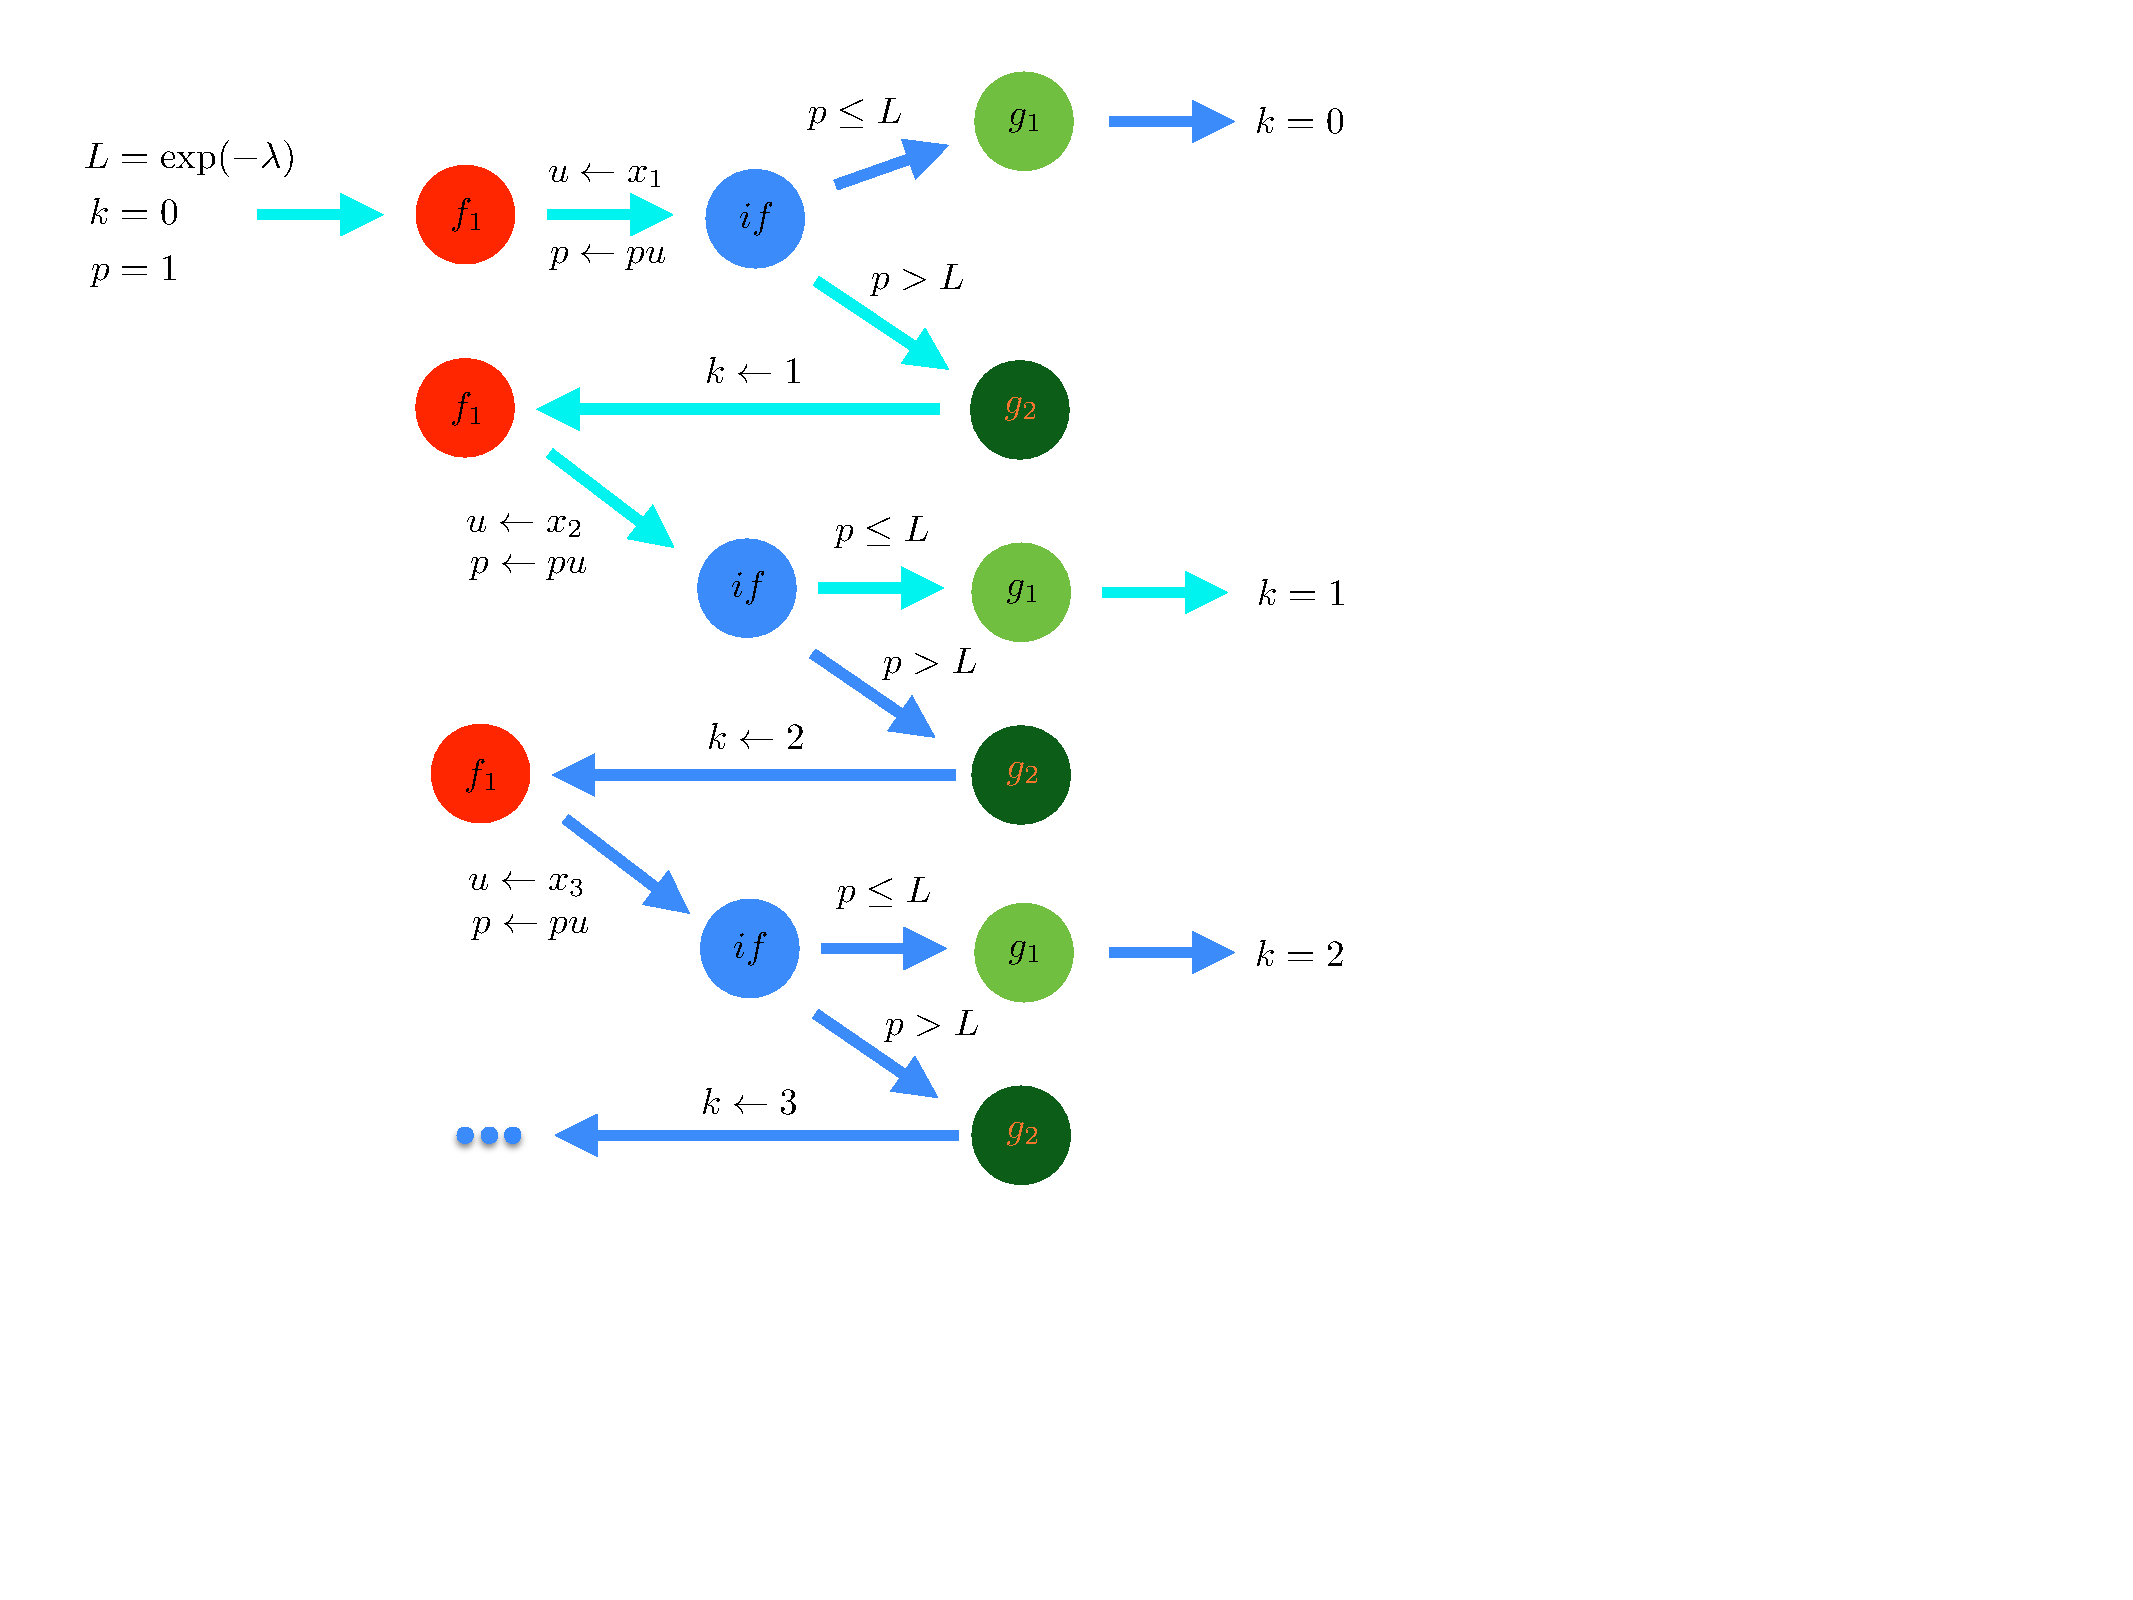
\includegraphics[width=0.75\textwidth]{probprog/figures/traces.pdf}			
					\subcaption{Possible traces for our query.  \sample statements are shown in red,
						\observe statements are shown in shades of green, and deterministic
						computations (given the outputs of the \sample statements) are shown in shades
						of blue.  Subscripts for the sample and observe statements show the lexical index
(i.e. $a_j \in \{1\}$ and $b_k\in\{1,2\}$), as do the different shades.  The cyan arrows correspond to
a particular execution path which gives output $k=1$ and has $n_x=2$, $n_y=2$, $b_1=2$, and $b_2=1$.
Valid traces for this particular path must have $x_1>\exp(-\lambda)$ and $x_2 \le \exp(-\lambda)/x_1$.
						\label{fig:probprog:poi-traces}
					}
	\vspace{10pt}
	\end{minipage}
		\begin{minipage}[b]{0.49\textwidth}
			\begin{algorithmic}[1]
				\renewcommand{\algorithmicrequire}{\textbf{Inputs:}}
				\renewcommand{\algorithmicensure}{\textbf{Outputs:}}			 
				\Require Event rate $\lambda$ 
				\State $L\leftarrow\exp(-\lambda)$, ~$k\leftarrow0$, ~$p\leftarrow1$
				\While{$p>L$}
				\State $u\leftarrow$\sample$(\textsc{Uniform}(0,1))$
				\State $p\leftarrow pu$
				\IIf{$p\le L$}; \textbf{break while}; \EndIIf
				\State \observe(\textsc{Bernoulli}(0.2), 1)
				\State $k\leftarrow k+1$
				\EndWhile
				\State \observe(\textsc{Bernoulli}(0.99),~$\mathbb{I}(k\text{>}3)$)
				\State \Return $k$
			\end{algorithmic}
			\subcaption{Query code for warped Poisson sampler\label{fig:probprog:poi-code}}
		\end{minipage}
				\begin{minipage}[b]{0.49\textwidth}
					\centering	~~
					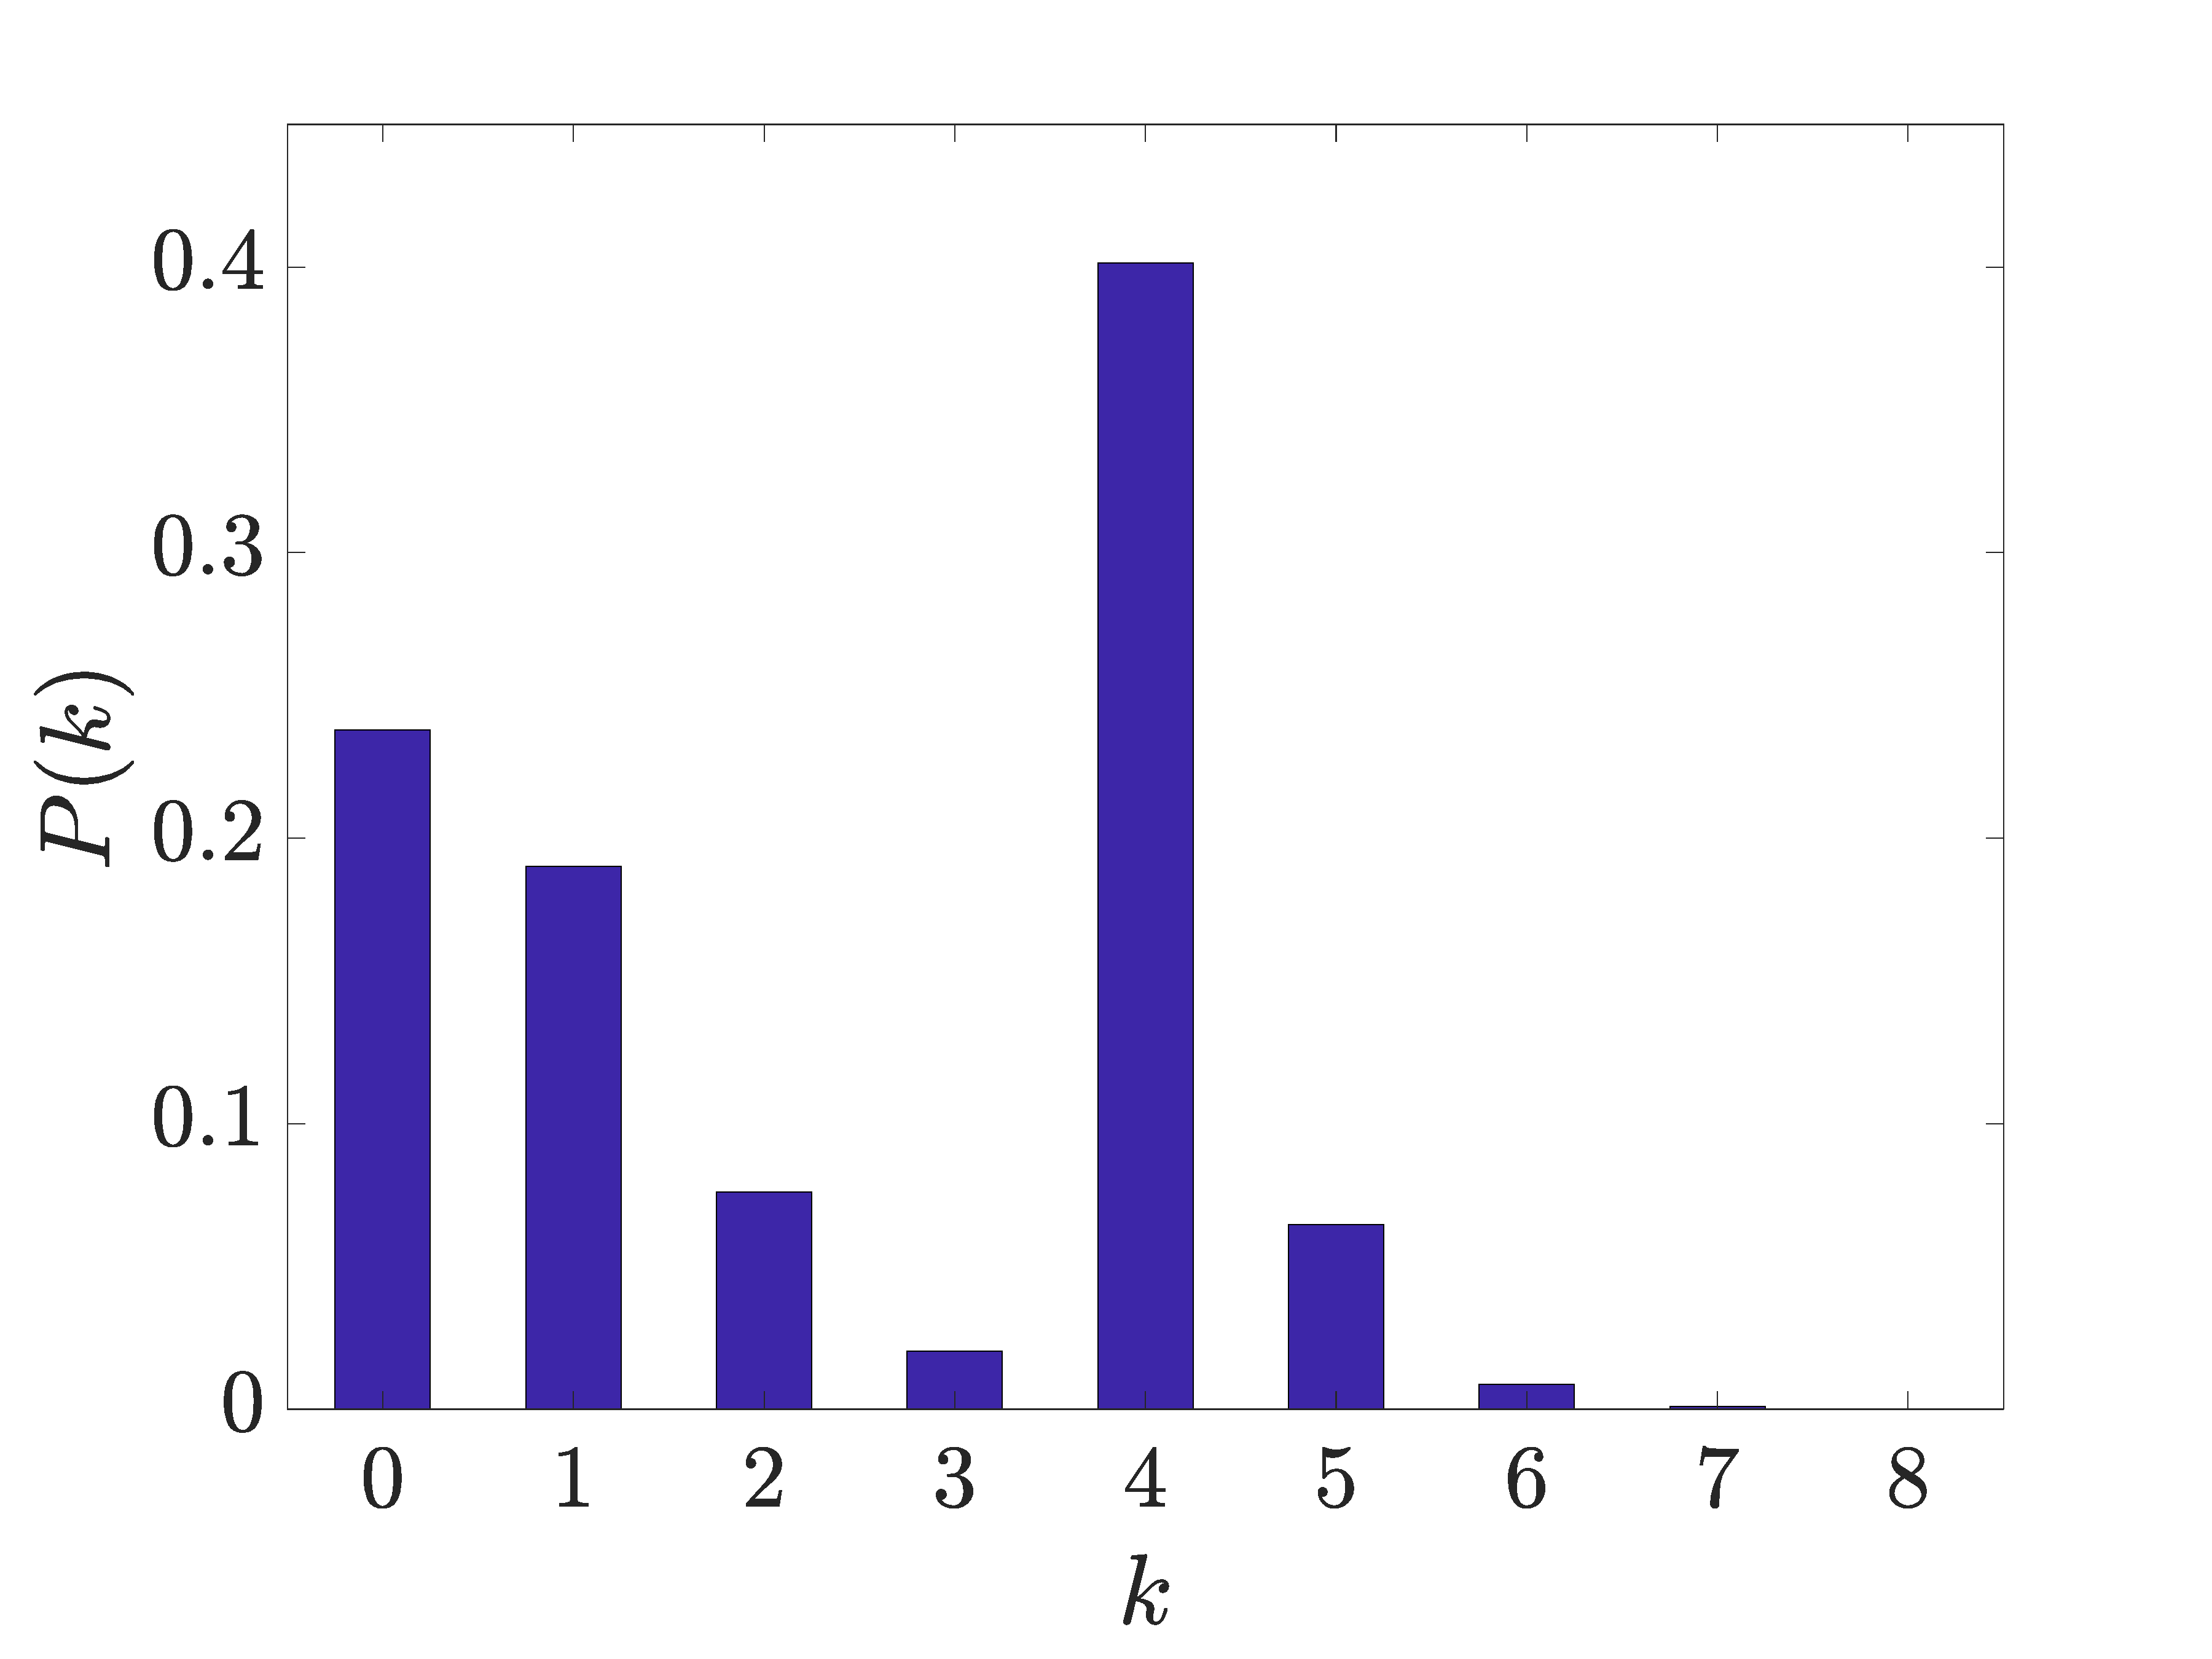
\includegraphics[width=0.95\textwidth]{probprog/figures/poisson_plot.pdf}			
					\subcaption{Conditional distribution on $k$ for $\lambda=4$.\label{fig:probprog:poi-res}
					}
				\end{minipage}
	\caption{Demonstration of stochastic execution traces using a warper
		Poisson sampler, adapted from~\cite[Figure 3.3]{paige2017thesis}.  The query defined in 
		\textbf{(b)} would output $k$ as per a Poisson
		distribution with event rate $\lambda$ if it were not for the \observe statements.
		As shown in \textbf{(c)} though, these \observe statements warp the distribution to
		give a lighter tail while discouraging $k\le3$.   Here both $n_x \in \mathbb{N}^+$ and
		$n_y \in \mathbb{N}^+$ depend on the trace and are unbounded.  Which
		\observe we see first is also probabilistic, while it some traces will be invalid, e.g. $x_{1:n_x}=[1,0.5]$
		as $x_1=1$ indicates there will be only a single \sample encountered.  Nonetheless, we can
		calculate the probability of a trace by following its path to completion while
		accumulating \sample and \observe factors.
		\label{fig:probprog:poisson}}
\end{figure}


An important point of note, is that, In general, $\gamma(x_{1:n_x}, \lambda)$ is not a normalized joint distribution.  This is firstly,
and most obviously, because $\lambda$ might contain terms, referred to as $\phi$ before, that are not
observed and so have no implied density.  Secondly, and more critically, even if $\phi = \emptyset$,
$\gamma(x_{1:n_x}, \lambda)$ is not necessarily correctly normalized, because of the ability to observe sampled variables and
condition the \sample statements on the observations.  As a simple example, our model
might consist of a $x_1 \leftarrow$\sample(\normal(0,1)) term followed by an \observe(\normal(-1,2),~$x_1$)
term.  This does not directly define any properly normalized joint distribution on any particular variables
(noting $\mathcal{N}(x_1;0,1) \mathcal{N}(x_1;0,2)$ is an unnormalized distribution with only the variable
$x_1$).  Consequently, there is no means of writing down a normalized joint distribution for a general
query in our universal PPL setup in closed form -- we might actually need to empirically estimate
the normalization constant to evaluate the joint.  This actually steps outside the conventional Bayesian
modeling framework and raises a number of interesting theoretical questions.  However, from a
practical perspective, we can note that provided the implicitly define normalization constant is finite,
the query also implicitly defines a correctly normalized conditional distribution (noting that
$\gamma(x_{1:n_x}, \lambda) \ge0$).
This is analogous to knowing the joint but not the posterior in Bayesian inference, though it is exactly
equivalent because the normalization constant is no longer the marginal likelihood.

As simple example of why it is important to be able to define models up to an unnormalized joint
distribution, consider an example where $a$ and $b$ are each sampled from discrete distributions
and we want to condition on the value of $a$ and $b$ being equal (see for example Figure~\ref{fig:probprog:schell}
in the next section).  Here
the combination of the sample statements and the observation that the two are equal clearly
does not lead to a correctly normalized joint (we do not even really have a conventional notion
of a likelihood), but it clearly defines an unnormalized conditional distribution as
\[
P(a,b | \mathbb{I}(a=b)) = \frac{P(a)P(b|a)\mathbb{I}(a=b)}{\sum_a \sum_b P(a)P(b|a) \mathbb{I}(a=b)}.
\]
In such cases where our observation is a hard constraint, we can view the normalizing constant for
the conditional defined by the query as the probability of our constraint being satisfied.  
For more general queries of discrete variables we might have, for example,
\[
P(x|\lambda) \propto f(x|\lambda)g(y=\kappa(x,\lambda)|x,\lambda)
\]
for some deterministic function $\kappa$.  Here we
can view the marginalization as being the probability of the event $y=\kappa(x,\lambda)$ under the joint $P(x,y)=f(x|\lambda)g(y|x,\lambda)$.
For our previous example we have $x:=a$, $y:=b$, $\kappa(a,\lambda):=a$, $f(a):=p(a)$, and $g(b=a):=p(b=a|a)$.
The same intuition applies to continuous cases where we now have the density of the event $y=\kappa(x,\lambda)$.
We can also think of $f(x|\lambda)g(\kappa(x,\lambda)|x,\lambda)$ as defining a unnormalized distribution on $x$ whose
normalization constant is $\int f(x|\lambda)g(\kappa(x,\lambda)|x,\lambda) dx$.  In general, our normalization
constant will be a combination of conventional marginal likelihood terms and contributions from these ``doubly defined''
terms. We refer to this normalization constant as the \emph{partition function}\footnote{Note this is not a
	term that is usually used in the probabilistic programming literature, where it is usually just referred to as a marginal
	likelihood.  Similarly, it is common in the literature to refer to a query as defining a ``normalized 
	joint'' density of $p_{\phi}(x_{1:n_x},y_{1:n_y}) = \prod_{j=1}^{n_x} f_{a_j}(x_j | \eta_j)
	\prod_{k=1}^{n_y} g_{b_k}(y_k | \psi_k)$.  We have deviated from both of these because, as our examples
	demonstrate, this viewpoint is technically a little questionable.  
%	For example, $p_{\phi}(x_{1:n_x},y_{1:n_y})$
%	defined in this way might not be a correctly normalized distribution and the normalization constant
%	for the conditional distribution might not be a true marginal likelihood.  
%	These distinctions will be
%	important in Chapters~\ref{chp:bopp} and~\ref{chp:nest} where we step outside the standard inference
%	framework.  
	For an even more rigorous treatment of the distributions defined by PPSs, we refer the reader to~\cite{staton2016semantics}. 
	} and note that it is given by
\begin{align}
\label{eq:probprog:mod}
Z(\lambda) &= \E \left[ \prod_{k=1}^{n_y} g_{b_k}(y_k | \psi_k) \middle| \lambda \right] = \int \gamma(x_{1:n_x},\lambda) dx_{1:n_x}\nonumber\\
&= \int_{x_{1:n_x} \in \{X : \mathcal{B}(X,\lambda)=1\}} 
\prod_{j=1}^{n_x} f_{a_j}(x_j | \eta_j) \prod_{k=1}^{n_y} g_{b_k}(y_k | \psi_k) dx_{1:n_x}
\end{align}
where the expectation is under running the query forwards (i.e. the distribution implied by simulating
from an equivalent query with all the \observe statements removed) and 
all terms in the integral are deterministically calculable for the query given $\lambda$ and $x_{1:n_x}$.
For our query to represent a well defined conditional distribution, it is necessary to have
$0<Z(\lambda)<\infty$.  Although $Z(\lambda)$ does not correspond exactly to a marginal likelihood,
we can still think of it in terms as representing a \emph{model evidence} in the same way, it just might
not be correctly normalized density in the same way a marginal likelihood is.

We now see that we can draw a direct analogy to the Bayesian framework whereby the product of the
\sample terms is analogous to the prior, the product of the \observe terms is analogous to the
likelihood, and the partition function is analogous to the marginal likelihood.  If observed variables
are not sampled within or used elsewhere in the query (e.g. being used a parameters in distribution objects
later used for sampling), then this analogy becomes exact as per our simplified setup.\footnote{Note that the
	observed variables should not be used in deterministic elements of the code for this to hold so that they
	cannot implicitly effect the sampling.}  However, as we have explained, it will often be desirable to go
beyond this framework to specify some models.  When we do, we still have an implicit Bayesian model, in the
same way that Bayes' rule means that a prior and a likelihood implicitly define a posterior, but we may not
actually have access to our implicitly defined prior and likelihood.

Given our query is now defined to specify a unnormalized conditional distribution rather than a normalized
joint distribution, it is natural to ask whether it is necessary for each \observe term to correspond to
a correctly normalized density for its output, instead of just restricting it to be a positive semi-definite
function representing an arbitrary soft constraint.  The answer is that it is not.  In fact, from a theoretical perspective,
it perhaps easier to not think of the distribution defined by the query as being a combination of sampling and conditioning terms,
but instead the product of the density of a correctly normalized generative
model and a positive semi-definite \emph{score function} that applies an unnormalized weighting to any possible
sample the generative model can produce.  This is
exactly the approach taken by~\citep{staton2016semantics} and~\citep{goodman_book_2014} who explicitly use such
score functions, calling them {\small \texttt{score}} and {\small \texttt{factor}} respectively.
We can also allow such functionality in our setup by defining a
special distribution class, \boppfactor, which can only be used with \observe, takes no parameters, and 
adds a factor to the trace probability equal to the exponentiation of the observed value.  Thus, for example, we could use
\observe (\boppfactor$(),\log(g(\psi)))$ to factor the trace probability by the output of the function $g(\psi)$.
The rationale for factoring by the exponentiation of the observed value rather than the observed value itself
is firstly to ensure that the factor is positive and secondly because it will be beneficial for
our system to work with log probabilities at its back-end to avoid numerical underflow issues.  Similarly
we will in practice specify distribution objects using there log densities.